\chapter{Model Selection}
\label{ch:ch4cv}

\section{Model selection}
We tried different families of classifier models. As an initial experiment, we simply divided the dataset into training and testing in a partition of 40\%-60\% and we evaluated all models commented in the previous chapter. Then, we selected some candidate models and we performed cross-validation reusing the code that we did for HW2 to tune the hyperparameters. The models with best results were the \verb|AdaBoostM1| with 6\%, the \verb|SVM| 6.5\%, and \verb|TreeBagger| with around 5\%, considering a trade-off between performance and running time. Then, with the tuning, the \verb|TreeBagger| classifier error was significantly lower that the other algorithms.

\section{Model hyperparameter selection}
The most significant hyperparameters relative to the classification error of the \verb|TreeBagger| were: 
\begin{itemize}
    \item[\textit{iter}] which in this case stands for the number of trees used for the random forests.
    \item[\textit{npred}] which is the number of predictor or feature variables to select at random for each decision split, as described in the previous section.
\end{itemize}
Also as hyperparameters, the following parameters related to the pre-treatment were considered: 
\begin{itemize}
    \item[\textit{minobs}] which was the minimum number of observations to create a dummy.
    \item[\textit{fm2}] which was a boolean variable representing whether to consider or not the order 2 feature map.
\end{itemize}

For the set of values described in the previous paragraph, a 2, 5 and 10-fold cross validation on the dataset was carried out. The best cross validation error was obtained with $iter = 500$, $npred = 100$, $minobs=70$, for any value of $fm$. For both of these, the error was in the order of $5,296\%$. We decided not to consider a feature map because of simplicity of the model. 

Computation times for cross-validation were high, so we decided to output partial results on an incremental \textit{.csv} file. A plot displaying the relationship between the \textit{iter} and \textit{npred} parameters with respect to the cv error is shown below: 

\begin{center}
  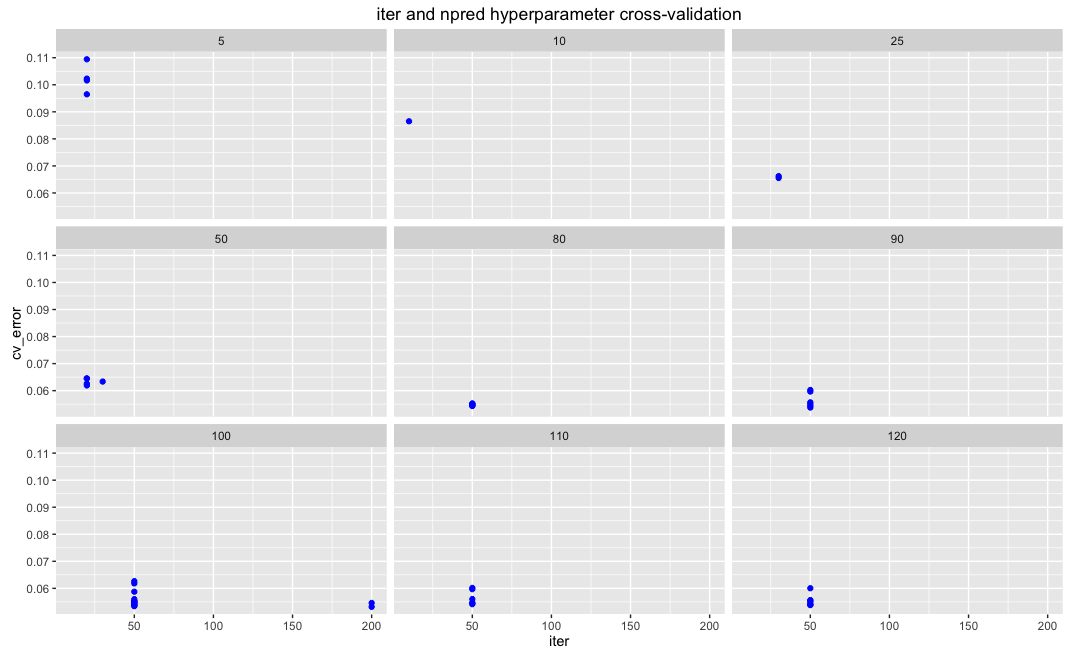
\includegraphics[scale=0.45]{./cv.png}
\end{center}    
